%!TEX root = ../../../FYP_Dissertation.tex

Knowing from the experience of the previous sections that lowering the
hierarchical depth would decrease the trace explosion. We tried to change the
object model slightly and leverage the trade off between the object model
flexibility and the performance. Figure \ref{fig:MO-alt-desc}, shows the tested
alternative design. It consists of separating variables from methods as in
general we declare methods in "classes" and data in "object" making the
redefinition of new function less frequent. This new approach makes all children
share the same \emph{methods} table until on instances tries to modify it,
performing then a copy-on-write. This means that accessing the methods of an
object is always done at the first level, lowering the need for hierarchical
chaining but it also means that the first \emph{\_\_index} function needs to
pay the price of an additional lookup when accessing data as there is no way
of knowing if a requested key reference a method or a data. So it needs to perform
a lookup to the \emph{methods} table first and in case of failure perform the
same hierarchical chaining as before. This new model on isolated test cases was
indeed performing better. Unfortunately it didn't help on average on the current
use of MAD as there is way more data fetched than methods. This model is still
kept up to date on a different development branch and might be reintroduced
depending on the evolution of MAD currently in development.

\begin{figure}
    \centering
    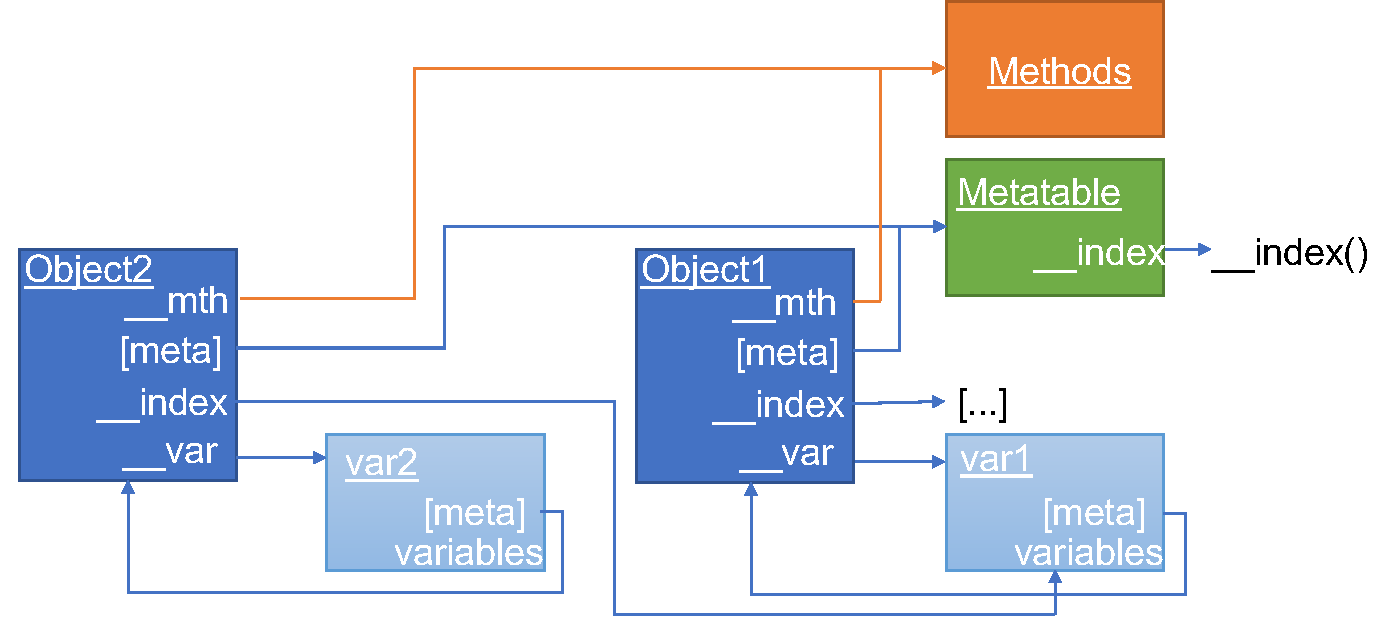
\includegraphics[width=\textwidth]{./Images/MO2.pdf}
    \caption{Alternative design of the model object}
    \label{fig:MO-alt-desc}
\end{figure}
